In this section we present a comparison between Casanova and other programming languages used for game development. The evaluation is based the on two essential aspects mentioned in Section \ref{sec:problem statement}: \textit{performance} and \textit{simplicity}. Performance is a fundamental indicator of the feasibility of a programming language that needs to be used in a resource-conscious scenario such as games. Simplicity is important as well, especially in those scenarios where development time and expense constitute a major concern (like for serious and indie game studios).


In particular we observe that, in many cases, programming languages for games offer a difficult either-or choice between simplicity and performance. As we will show, Casanova solves this apparent dichotomy by offering both at the same time.
\subsection{Tested languages}
\label{Languages tested}
We have chosen four languages which represent various development styles and which are all used in practice for building games. We have mostly focused on those languages which are used for building game logic, and we have shied away from considering languages (such as C++) which are used for building engines or libraries \cite{gregory2009game}, as Casanova is not ``competing'' with them. Three of the chosen languages are dynamically typed programming languages: Lua, JavaScript, and Python, which have as their main selling points simplicity and immediacy \cite{gutschmidt2004game}. The fourth chosen language is C\# because of its good performance and relative simplicity. One could argue that we are comparing our language, which might appear as a Domain Specific Language (DSL), with General Purpose Languages (GPL's). However, Casanova 2 is actually a GPL, although its main field of application is computer game development.

The ``benchmark sample'' simulates a game with ten thousands patrols. We made an effort towards implementing the sample by using coroutines and generators \cite{marlin1980coroutines} whenever available, in order to express the game logic in an idiomatic style for each language. In order to compare the language functionality, we are only running the logic of the game and we do not execute any other component unrelated to it (such as the graphics engine), to produce a fair performance benchmark. The code samples can be found on \cite{codeplexSource}.

%The chosen languages are:
%\begin{itemize}
%\item \textbf{Lua}: writing games with Lua is quite straightforward. Its compactness allows developers to easily embed it into complex systems. Its support for coroutines and simple API allows for fast prototyping, especially when expressing behaviours which depend on time. This makes Lua suitable for building games and in particular for scripting. Lua has been used in various commercial games, and engines \cite{LUAgames}.
%\item \textbf{JavaScript}: a widely used language \cite{JavaScriptgames}. Its immediate syntax and compactness make it relatively easy to learn. Games built with JavaScript can be run in web-browsers. This has made JavaScript a popular choice among developers.
%\item \textbf{Python}: a widely used scripting language for games. Python offers a huge set of libraries. It also features specific constructs, such as generators, for managing the flow of time, for greatly simplifying the task of building state machines. Several games, and engines \cite{PYTHONgames}, were built using Python.
%\item \textbf{C\#}: a high-performance oriented language used by many developers for writing games and engines. It has been widely and successfully used for games and engines \cite{CSHARPgames}.
%\end{itemize}

\subsection{Performance}
We have generated tens of thousands of entities in a loop that simulated a hundred thousand frames. This corresponds roughly to half an hour of play time on a reasonably crowded scene. The results are summarized in Table \ref{Performance comparison - Time per frame}.

\begin{table}[!t]
\caption{Performance comparison}
\label{Performance comparison - Time per frame}
\centering
\begin{tabular}{|c||c|}
\hline
Language & Time per frame\\
\hline
Casanova & 0.07ms\\
\hline
C\# & 0.12ms\\
\hline
JavaScript & 24.07ms \\
\hline
Lua & 20.90ms\\
\hline
Python & 20.15ms \\
\hline
\end{tabular}
\end{table}

As we can see from the table, the performance of Casanova 2 is of the same order as C\#, and is multiple orders of magnitude faster than that of the scripting languages.
In this simple but populated scenario, the limits of Lua, Python, and JavaScript, deriving from the high cost of dynamic lookup, are clearly shown. In addition, all languages use virtual calls to methods, such as those for managing and executing coroutines and generators, which add overhead at the expense of performance.
In short, Casanova 2 generates highly optimized rule code which does not require general purpose constructs, such as coroutines in games, that often use virtual methods and dynamic lookups. In a sense, Casanova 2 uses all the static information it can to avoid work at runtime.


We believe that it is worthy of notice how much Casanova in this prototypical implementation offers a performance which is even better than that of a very high quality and mature compiler such as that of C\#.


\subsection{Ease of use}
Assessing the simplicity of a programming language is a daunting task. Just as much as beauty lies in the eye of the beholder, simplicity in programming languages heavily depends on the programmer preferences, history, and previous knowledge. %For this reason we present here some evaluation of how simple Casanova is, while at the same time openly acknowledging the herculean difficulty of the task. We have assessed difficulty through a comparison between various languages, and we have also conducted a standalone user study among a series of students.

For the comparison we have taken the benchmark sample and implemented it with each of the considered languages. In order to assess the complexity of the sources we have:
\begin{enumerate}
\item counted the number of lines of each source, thereby assessing the size of the implementation, with the assumption that a bigger sample corresponds to more complexity;
\item counted the number of keywords and operators (syntagms) that come into play for each implementation, with the assumption that a high count corresponds to more required knowledge from the developer.
\end{enumerate}

\begin{table}[!t]
\caption{Syntax comparison}
\label{Syntax languages comparison}
\centering
\begin{tabular}{|c||c||c||c|}
\hline
Language & Syntagms & Lines of code & Total words\\
\hline
Casanova & 47 & 31 & 104\\
\hline
C\# & 61 & 69 & 269\\
\hline
JavaScript & 52 & 41 & 257\\
\hline
Lua & 47 & 45 & 249\\
\hline
Python & 50 & 34 & 214\\
\hline
\end{tabular}
\end{table}
The results are summarized in Table \ref{Syntax languages comparison}. As we can see, Casanova 2 resulted in significantly less lines of code and syntagms, especially with respect to C\# (the only other language with comparable high performance).


\begin{figure*}[!t]
\centerline{\subfloat[Dyslexia]{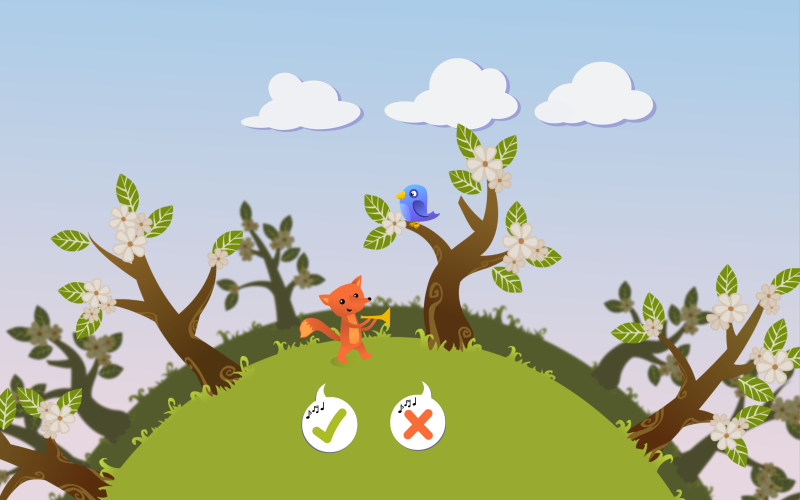
\includegraphics[width=2.0in]{Figures/dyslexia_game.png}%
\label{Dyslexia game}}
\hfil
\subfloat[RTS]{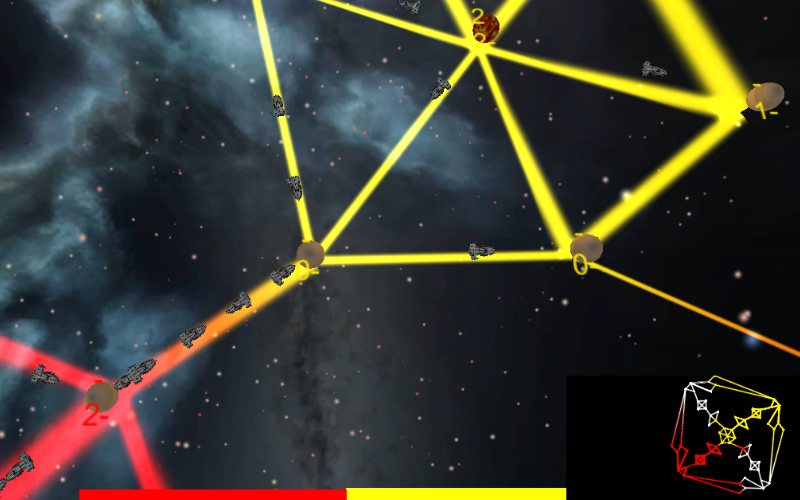
\includegraphics[width=2.0in]{Figures/rts.png}%
\label{RTS game}}}
\caption{Casanova games}
\label{casanova_games}
\end{figure*}



\subsection{Summary}
In conclusion, Casanova 2 has been shown to offer both good performance and simple code at the same time. On the one hand, Casanova 2 is as simple as ``easy to use''  scripting languages. On the other hand, this simplicity does not come with the usual associated hit in performance that characterizes these languages. The performance of Casanova is even a bit better than that of C\#, a highly optimized commercial language. A series of applications has been built with the language as part of teaching and research projects.  One of those is an RTS game (see Figure \ref{RTS game}) that features complex integration with a professional-quality engine, Unity3D\cite{Unity3D}. The other notable application is a game for detecting dyslexia in children (see Figure \ref{Dyslexia game}). The game is currently being used as a tool for research and features some articulated animations and state machines. These applications can be found at \url{http://casanova.codeplex.com/}.

% Here, for instance, you could mention the games for which you have screenshots. 